\documentclass[a4paper,11pt]{report}
\usepackage[spanish,mexico]{babel}
\usepackage[utf8]{inputenc}
\usepackage[T1]{fontenc}
\usepackage{amsmath,bm}
\usepackage{enumitem}
\usepackage{amssymb}
\usepackage{wasysym}
\usepackage[dvipsnames,pdftex]{color}
\usepackage[x11names]{xcolor}
\usepackage{tikz, tkz-euclide}
\usepackage[american]{circuitikz}
\usepackage{siunitx}
\usetikzlibrary{arrows}
\usepackage{textcomp}
\usepackage[colorinlistoftodos]{todonotes}
%\usepackage[left=2cm,right=1.5cm,top=1cm,bottom=1cm]{geometry}
%\usepackage{helvet}
%\renewcommand{\familydefault}{\sfdefault}
\setlength{\oddsidemargin}{0in}
\usepackage{geometry}
\geometry{total = {180mm,270mm},
			left = 20mm, top = 20mm,
            right=10mm,bottom=20mm,%
            footskip=10mm}
\usepackage{float} 
% \setlength{\topmargin}{0in}
% \setlength{\voffset}{-0.5in}
% \setlength{\hoffset}{0.3in}
% \setlength{\textheight}{700pt}
% \setlength{\textwidth}{440pt}
% \setlength{\topskip}{0in}
% \setlength{\parskip}{2ex}
 \renewcommand{\baselinestretch}{1.2}
\usepackage{diagbox}
\usepackage{array}
\usepackage{listings}
\usepackage{caption}
%%% comandos definidos por el usuario
\begin{document}
\setcounter{page}{1}
\pagenumbering{roman}
\thispagestyle{empty}
\begin{center}
{\huge UNIVERSIDAD NACIONAL DE INGENIERÍA}\\[0.9cm]
{\Large FACULTAD DE INGENIERÍA MECÁNICA}\\[0.6in]
\end{center}
\begin{figure}[h]
\begin{center}

\includegraphics[scale=0.33]{logoUNI.png}
\vspace{0cm}
\end{center}
\end{figure}
\vspace{0.5cm}
\begin{center}
INFORME DE LABORATORIO\\
LABORATORIO DE CIRCUITOS ELÉCTRICOS\\[5mm]
{\large MEDIDA DE LA INDUCTANCIA MUTUA EN UN CIRCUITO ACOPLADO MAGNÉTICAMENTE}\\[10mm]
\vfill
LIMA - PERÚ \hfill OCTUBRE 2019
\end{center}
\newpage
\thispagestyle{empty}
\begin{center}
{\Huge MEDIDA DE LA INDUCTANCIA MUTUA EN UN CIRCUITO ACOPLADO MAGNÉTICAMENTE}\\[0.7cm]
\small ENTREGADO:\\[0.05cm]
\small 30 OCTUBRE 2019\\[1.2cm]
\end{center}
\begin{flushleft}
{\large ALUMNO:}\\[2cm]
\end{flushleft}
%\begin{center}
%\begin{tabular}{c@{\hspace{0.5in}}c}
%\rule[1pt]{3.14in}{1pt}\\
%Sotelo Cavero Sergio, 20172125K% & Nombre 5, 2017 \\[1.5cm]
%\end{tabular}
%\end{center}
\begin{center}
\begin{tabular}{c@{\hspace{0.6in}}c}
\rule[1pt]{3.14in}{1pt}\\
Huaroto Villavicencio Josué, 20174070I \\[2cm]
%\rule[1pt]{3.14in}{1pt}\\
%Landeo Sosa Bruno, 20172024J \\[2cm]
%\rule[1pt]{3.14in}{1pt}\\
%Quesquén Vitor Angel, 20170270C \\[2cm]
%\rule[1pt]{3.14in}{1pt}\\
%Sotelo Cavero Sergio, 20172125K \\[2cm]
\end{tabular}
\end{center}
%\begin{center}
%\begin{tabular}{c}
%\rule[1pt]{3.14in}{1pt}\\
%Huaroto Villavicencio Josué, 20174070I \\[2.5cm]
%\end{tabular}
%\end{center}

%\rule[1pt]{3.14in}{1pt}\\
%Maguiña Amaya Wladimir, 20172019F \\[3cm]
%\rule[1pt]{3.14in}{1pt}\\
%Luis Sosa Jose, 19774147I \\[3cm]
%\rule[1pt]{3.14in}{1pt}\\
%Sotelo Cavero Sergio, 20172125K
%\end{tabular}
%\end{center}
%\\[0.7cm]
{\large PROFESOR:} \\[2cm]
\begin{center}
\begin{tabular}{c}
\rule[3pt]{4.8in}{1pt}\\[1pt]
ING. SINCHI YUPANQUI, FRANCISCO 
\end{tabular}
\end{center}
\vfill
%\newpage
%\begin{center}
%{\Large \bf{RESUMEN}}
%\end{center}
\newpage
\tableofcontents
%\listoffigures
%\addcontentsline{toc}{chapter}{Índice de figuras}
\newpage
\pagenumbering{arabic} %%% esto es para regresar el modo de numeración a numeración arábiga
\setcounter{page}{1}  %%% empezamos en página 1
%\part{Introducción}
\chapter{Objetivos}
\begin{enumerate}
\item Determinar el coeficiente de acoplamiento magnético ``k'' y la inductancia mutua ``M'' en dicho circuito.
\item Analizar y evaluar el acoplamiento magnético que existe en un circuito acoplado.
\end{enumerate}
\chapter{Acoplamiento de inductancias}
Cuando fluye una corriente constante en una bobina como en la ilustración de la derecha, se produce un campo magnético en la otra bobina. Pero como el campo magnético no está cambiando, la ley de Faraday nos dice que no habrá voltaje inducido en la bobina secundaria. Pero si abrimos el interruptor, para interrumpir la corriente como en la ilustración del medio, habrá un cambio en el campo magnético de la bobina de la derecha y se inducirá un voltaje. Una bobina es un dispositivo reaccionario; ¡no le gusta ningún cambio!. El voltaje inducido hará que fluya una corriente en la bobina secundaria, que trata de mantener el campo magnético que había allí. El hecho de que el campo inducido siempre se oponga al cambio, es un ejemplo de la ley de Lenz. Una vez que ya se ha interrumpido la corriente y se cierra el interruptor para hacer que fluya de nuevo la corriente como en el ejemplo de la derecha, se inducirá una corriente en dirección opuesta, para oponerse al incremento del campo magnético. La persistente generación de voltajes que se oponen al cambio en el campo magnético es el principio de operación de un transformador. El hecho de que el cambio en la corriente de una bobina, afecte a la corriente y el voltaje de la segunda bobina, está cuantificado por una propiedad llamada inductancia mutua.
\begin{figure}[H]
\centering
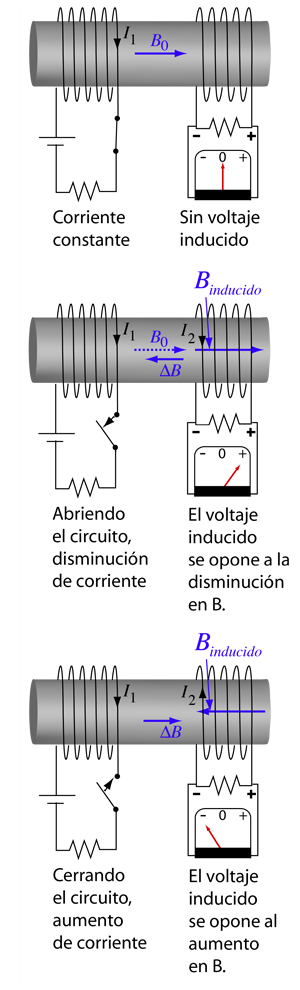
\includegraphics[height=11cm, width=7cm]{indmut.png}
\end{figure}
\chapter{Inductancia mutua}
Se llama inductancia mutua al efecto de producir una fem en una bobina, debido al cambio de corriente en otra bobina acoplada. La fem inducida en una bobina se describe mediante la ley de Faraday y su dirección siempre es opuesta al cambio del campo magnético producido en ella por la bobina acoplada (ley de Lenz ). La fem en la bobina 1 (izquierda), se debe a su propia inductancia L.\\
La fem inducida en la bobina \#2, originada por el cambio en la corriente I$_{1}$ se puede expresar como:
$$
\mathrm{FEM}_{2} = -N_{2}A\frac{\Delta B}{\Delta A} = -M\frac{\Delta I_{1}}{\Delta t}
$$
La inductancia mutua M se puede definir como la proporción entre la fem generada en la bobina 2, y el cambio en la corriente en la bobina 1 que origina esa fem. La aplicación mas usual de la inductancia mutua es el transformador.
\chapter{Circuitos acoplados}
Con frecuencia el flujo a través de un circuito varía con el tiempo como consecuencia de las corrientes variables que existen en circuitos cercanos. Se produce una fem inducida mediante un proceso que se denomina inducción mutua.
\begin{figure}[H]
\centering
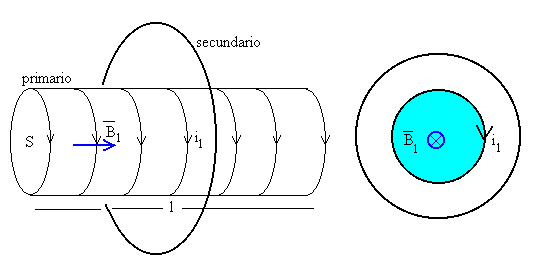
\includegraphics[scale=0.8]{Acoplados1.png}
\end{figure}
\section{El transformador}
Hace algo más de un siglo que se inventó este dispositivo que ha hecho posible la distribución de energía eléctrica a todos los hogares, industrias, etc. Si no fuera por el transformador tendría que acortarse la distancia que separa a los generadores de electricidad de los consumidores. \\
El transformador lo encontramos en muchos lugares, en las lámparas de bajo consumo, cargadores de pilas, en sótanos de edificios, en las centrales hidroeléctricas y otros generadores de electricidad. Su tamaño puede variar desde muy pequeños a enormes transformadores que pueden pesar más de 500 Tm.
\begin{figure}[H]
\centering
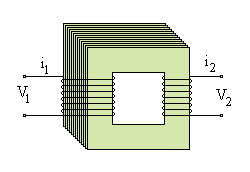
\includegraphics[scale=1.1]{Acoplados2.png}
\end{figure}
El primario y el secundario de un transformador tienen el mimo núcleo de hierro que asegura que el flujo a través de cada espira sea el mismo.
$$
\frac{V_{2}}{V_{1}} = \frac{N_{2}}{N_{1}}
$$
\begin{thebibliography}{99}  %%%este es un contador para el número de bibliografías utilizados.
\addcontentsline{toc}{chapter}{Bibliograf\'{\i}a} %%% Para introducir la bibliografía en el índice.
%\bibitem{Rahman}{Rahman,Aminur y Doe, Hidekazu; ``Ion transfer of tetraalkylammonium cations at an interface between 
%frozen aqueous solution and 1,2-dichloroethane".{\em{Journal of Electroanalytical Chemistry}} {\bfseries 424},159,(1997).}
\bibitem{Gro}{Boylestad, Robert M. ``Introducción al análisis de circuitos''. {\em{Pearson}}}
\bibitem{Gro}{Sadiku, Matthew N. ``Fundamemtos de circuitos eléctricos''. {\em{Mc Graw Hill}}}
%\bibitem{Ding}{Ding, Zhifeng. ``Spectroelectrochemistry and photoelectrochemistry of charge transfer at liquid/liquid
%interfaces". {\em {Tesis, EPFL,}}(1999).}
%\bibitem{AL}{Alonso, Jose M. \em{Técnicas de mecanizado 1}}
%\bibitem{AL}{Alonso, Jose M. ``Técnicas de mecanizado 1". {\em{Paraninfo}} {\bfseries España-Madrid}, 6-20, (2001).}
%\bibitem{Samec2}{Samec Z., Lhotsky A., Jänchenová H., y Marecek, V. ``Interfacial tension and impedance measurements
%of interfaces between two inmiscible electrolyte solutions". {\em{Journal of Electroanalytical Chemistry}} {\bfseries
%43}, 47, (2000).}
%\bibitem{Day}{Day R.A. y Underwood A.L. {\textit{Química Analítica Cuantitativa}},5ºed. Prentice-Hall, México, 1998. 45-48.}
%\bibitem{Keyser}{Farah Abud, Michel. ``Determinación de la vida útil en herramientales de corte endurecido por el proceso de borurización en pasta''. {\em{Instituto tecnológico y de estudios superiores de Monterrey}}}
%\bibitem{Zolotorevski}{Escalona, I. ``Máquinas: herramientas por arranque de viruta.''.{\em{El Cid Editor.}}}
%\bibitem{Lasheras}{Lasheras. ``Tecnología de los Materiales Industriales''.} 
%\bibitem{Dieter}{Dieter. ``Metalurgia mecánica''.}
%\bibitem{Apraiz}{Apraiz, J. ``Tratamiento Térmico de los Aceros''.}
%\bibitem{Smith}{Smith, William F. y Ph.D. Hashemi, Javad ``Ciencia e ingeniería de materiales". {\em{
%Madrid: McGraw-Hill, Interamericana de España.}} 570, (2004).} 
%\bibitem{Callister}{Callister, William D. y Rethwisch, David G. ``Introducción a la ingeniería de los materiales''. %{\em{Barcelona Reverté.}}, 960, (2007).} 
%\bibitem{Askeland}{Askeland, Donald R., Pradeep P. Phulé y Wright, Wendelin J. ``Ciencia e ingeniería de los materiales''.{\em{México, D.F. Internacional Thomson Editores.}} {\textit{$6^{ta}$ edición}}, 1004, (2012).}
%\bibitem{HARDBANDING}{Tabla de conversión de escala de durezas. \begin{verbatim}http://%hardbandingsolutions.com/postle_sp/hardness.php
%\end{verbatim}}
%\bibitem{HE}{Fresadora. \begin{verbatim} http://lizdenbow.blogspot.com/
%\end{verbatim}}
%\bibitem{ASTM}{Normas ASTM.}
%\bibitem{NTP}{Normas NTP.}
\end{thebibliography}
\end{document}